\documentclass[a4paper,12pt]{extarticle}
\usepackage[margin=1.5cm]{geometry}
\usepackage{amsmath, amssymb}
\usepackage{array}
\usepackage{multicol}
\usepackage{helvet}
\usepackage{multirow}
\usepackage{graphicx}
\renewcommand{\baselinestretch}{2}
\renewcommand{\familydefault}{\sfdefault}

\begin{document}

    \begin{tabular}{| c | c | c | c |}
        \hline
        & MATEMÁTICAS & 05/03/2026 & calificación \\
        \hline 

        \multirow{2}{*}{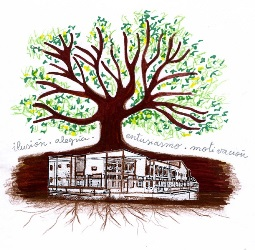
\includegraphics{../../img-Logos/iesoGalileo.jpg}} & Nombre y apellidos \hspace{120pt} & Ex. 2º ESO UD5:  & \\ 
        &&Ecuaciones& \\ 
        \hline
    \end{tabular}
    
    \begin{tabular}{| l | }
        \hline
        NOTAS: \\ 
            1. El examen tiene que ser limpio, ordenado y sin faltas de ortografía. \\
            
            2. El examen ha de realizarse en bolígrafo negro o azul, evitando tachones en la medida \\
            de lo posible. \\ 
            
            3. Deben aparecer todas las operaciones NO vale con indicar solo el resultado.\\
            
            4. Los problemas deben contener: Datos, planteamiento y resolución, respondiendo a lo \\
            que se pregunte, NO vale con indicar un número como solución del problema.\\

            5. Persona que se vea copiando o hablando con un compañero tiene un cero en el examen\\

            6. NO está permitido el uso de calculadoras \\
        \hline
    \end{tabular}

    \begin{enumerate}
        \item (1 punto) Determina los miembros, los términos y el grado de la ecuación.
             \[5x-2 = x^2 +4\]
                    \begin{itemize}
                        \item miembros: 
                        \item términos:
                        \item grado: 
                    \end{itemize}
            
        \item (2 puntos) Resuelve la ecuación de primer grado:
            \[x-(x+2)-3(x+1)=4-2(x+1)\]
            $\vspace{5cm}$ 
        \item (1 punto) Resuelve la ecuación de segundo grado: 
            \[x^2-5x+6=0\]
        \item (1 punto) Resuelve la ecuación de segundo grado incompleta
            \[x^2-5x+6=0\]
        \item (1 punto) Resuelve la ecuación de segundo grado incompleta 
            \[x^2-16=0\]
        \item (2 puntos) La edad de una madre es el triple que la de su hija.  Si dentro de 4 años la edad de la madre será el doble que la de la hija, ¿cuál es la edad actual de cada una? $\vspace{4cm}$ 
        \item (2 puntos) La suma de tres números consecutivos es 45. Hállalos. $\vspace{4cm}$ 
        \item (EXTRA) Un rectángulo mide 4 cm más de largo que de ancho, y su área es de 96 $cm^2$. ¿Cuánto miden sus lados?
    \end{enumerate}
\end{document}